%MARCOS RIAL DOCAMPO
%Parte del documento principal TFG

%%%%%%%%%%%%%%%%%%%%%%%%
%% MATERIAL Y MÉTODOS %%
%%%%%%%%%%%%%%%%%%%%%%%%


\chapter{Material y métodos}
\label{cap:materialymetodos}

\section{Estudio radiométrico}
En este caso, obtendremos del estudio radiométrico firmas espectrales del tipo monobanda. Estas se caracterizan porque la respuesta de los objetos analizados es contenida en un solo canal continuo de datos \citep{andinofase1}.%\Sep

La meteorología y la difícil accesibilidad de la zona hicieron aconsejable hacer una toma de muestras y realizar la observación en un estudio. El material vegetal utilizado en el estudio fueron muestras recientes de hojas tomadas de árboles de cada especie como se describe en la metodología de obtención de firmas espectrales de \cite{andinofase2} y como se puede apreciar en las figuras \ref{fig:mangle_recolectado} y \ref{fig:curva_espectral}.

\begin{figure}
	\centering
	\includegraphics[width=0.9\linewidth]{./Imagenes/Mangle_recolectado.eps}
	\captionsetup{font={footnotesize,it}}
	\caption[Mangle recolectado]{Hojas de las especies de mangle a analizar. Fotografía de Rafael Corrales.}
	\label{fig:mangle_recolectado}
\end{figure}

\begin{figure}
	\centering
	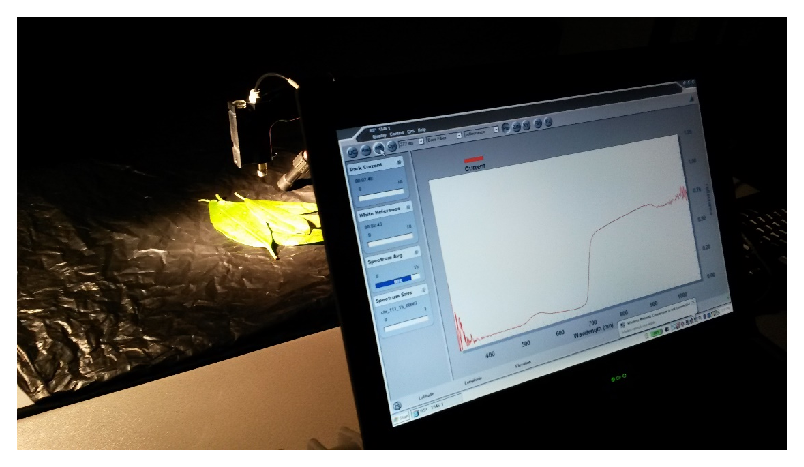
\includegraphics[width=0.9\linewidth]{./Imagenes/Curva_espectral.eps}
	\captionsetup{font={footnotesize,it}}
	\caption[Obtención de firmas]{Momento de la obtención de las firmas espectrales de una especie. Fotografía de Rafael Corrales.}
	\label{fig:curva_espectral}
\end{figure}

\subsection{Datos}\label{subsec:datos}
Los datos obtenidos por el profesor Rafael Enrique Corrales con el espectro-radiómetro de campo se presentan en cuatro archivos de extensión .dat de texto simple, uno para cada especie más uno del conjunto que no se utilizará.%\Sep

La característica principal de estos datos es que abarcan un amplio rango espectral de forma continuada, similar a lo que ocurre en la obtención de una imagen, pero en este caso los datos serían solamente de un punto, no de una superficie extensa. El rango espectral captado por el espectro-radiómetro comprende de 324.5 - 1075,5 nm almacenando la reflectividad media para intervalos de onda de 1nm.%\Sep

Simultáneamente a la toma de datos se visitaron puntos donde era conocida la existencia de mangle (cuadro \ref{tab:puntos}). Estos estrictamente no son puntos de control porque no se trata de puntos en los que no solo existe la cobertura de un tipo de mangle concreto sino que pueden confluir varias cubiertas en el mismo punto. En ellos se observaron la certeza del cambio en la existencia de mangle y alguna de las causas que lo motivan, como la presencia de salineras y estanques de camarón. En algunos casos, como el de La Brea la presencia de R. mangle es para reducir el impacto visual de las camaroneras. En otras zonas como en Los Ganchos, la pérdida de cobertura de mangle es debida a la dinámica de la costa provocada por la desembocadura del río Nacaome.

\begin{table}[ht]
	\centering
	\begin{tabular}{@{}ccll@{}}
	\toprule[0.4mm]
	East & North & Nombre & Epecies existentes\\
	\midrule
	452379 & 1476560 & Pasadero de los Pericos & \textit{R. mangle}.\\
	450493 & 1476503 & Punta de los Elotes & \textit{R. mangle} y \textit{L. racemosa}\\
	448571 & 1484829 & Corinto & \textit{R. mangle} y \textit{L. racemosa}\\
	438047 & 1488915 & Jiote Grande & \textit{R. mangle}, \textit{L. racemosa} y \textit{A. germinans}\\
	434163 & 1487386 & Los Ganchos & \textit{R. mangle}\\
	440251 & 1489561 & La Brea & R. mangle, \textit{L. racemosa} y \textit{A. germinans}\\
	\bottomrule[0.4mm]
	\end{tabular}
	\captionsetup{font={footnotesize,it}}
	\caption[Puntos de control]{Serie de puntos conocidos de existencia de manglar con la especie predominante.}
	\label{tab:puntos}
\end{table}

\section{Software} \label{sec:software}
El uso de software libre en general es un recurso a tener en cuenta para realizar trabajos técnicos que utilizan un componente informático \citep{MatellanOliveira2004} \citep{Mas2005software}. En concreto es uso de este tipo de software en trabajos sobre recursos medioambientales cobra importancia principalmente por, entre otras cosas:

\begin{enumerate}
	\item Abarata el coste del proyecto al ser bajo o nulo el coste de una licencia de uso.
	\item Cuenta con un buen soporte y servicio técnico llevado en algunos casos por comunidades de usuarios y a largo plazo. Se evita la obsolescencia del producto.
	\item Formatos estandarizados que permiten la interoperabilidad.
	\item Se centra en proporcionar un servicio y no un producto.
\end{enumerate}

Este \ac{TFG} se ha hecho íntegramente con software libre distribuido bajo licencia GNU GPL salvo que se indique lo contrario, utilizando los programas seguidamente mencionados sobre un sistema operativo GNU/Linux, en concreto sobre la distribución Ubuntu 14.04\footnote{\url{http://www.ubuntu.com/}}.%\Sep

Adicionalmente se ha hecho un control de versiones remoto con el software Git\footnote{Otra opción en lo que a control de versiones se refiere sería la del software \ac{SVN} \citep{Latex2011} pero este solamente permite hacer un control local de los cambios.} que, mediante repositorios, permite gestionar un historial de ficheros y carpetas recordando y organizando el contenido en cada momento documentando los cambios que ha sufrido y quién y por qué los ha realizado. Permite, por tanto, recuperar el documento a versiones anteriores o revisar el proceso de desarrollo del mismo funcionando como respaldo. De esta forma se permite el acceso a los archivos por la plataforma web GitHub de forma pública\footnote{El código de este trabajo es accesible desde la página web \url{https://github.com/MarcosRial/TFG}}. La interfaz gráfica utilizada ha sido SmartGit\footnote{\url{http://www.syntevo.com/smartgit/}} \citep{GmbH2015} libre y de uso gratuito para fines no comerciales y donde se pueden hacer cómodamente la mayoría de las operaciones de control de cambios.%\Sep

\paragraph{R}
Para el tratamiento de los datos se ha utilizado el software estadístico de uso libre R Project for Statistical Computing, más conocido como R\footnote{\url{http://www.r-project.org/}} \citep{R2013} en su versión 3.2.0. R puede definirse como un software de análisis estadísticos, como un generador de gráficos o como un lenguaje de programación. Si bien es un software pensado para su uso sobre interfaces de código, para la realización de este \ac{TFG} se ha utilizado la interfaz gráfica del software libre RStudio\footnote{\url{https://www.rstudio.com/}}, bajo licencia AGPL, con el fin de hacer que su uso resulte más amigable.%\Sep

R, como la mayoría de software que funciona sobre sistema operativo GNU/Linux, se compone de módulos o paquetes que se incorporan a una base del programa, llamado \textit{R core}, para extender sus posibilidades y funciones. Actualmente el número de paquetes de R existentes ronda los 4000, desarrollados por usuarios y programadores de todo el mundo. Esta cifra se incrementa ya que periódicamente se suben paquetes a la red de repositorios oficial \ac{CRAN}\footnote{\url{http://cran.r-project.org/}}.%\Sep

R es uno de los lenguajes más utilizados en estadística. Adicionalmente abarca otros muchos campos debido a la cantidad de librerías disponibles como tratamiento de imágenes satélite o clasificación supervisada.

\paragraph{GRASS GIS}
Para el tratado de imágenes Landsat y su posterior clasificación se utiliza el programa de \ac{SIG} gratuito y de código abierto \ac{GRASS}\footnote{\url{http://grass.osgeo.org/}} \citep{GRASS_GIS_software}. GRASS es un proyecto de la \ac{OSGeo}. Es un potente software en lo que a utilización de manejo y análisis de información geoespacial se refiere. Su funcionalidad es similar a otros programas \ac{SIG} como QGIS\footnote{\url{http://www.qgis.org/es/site/}}, en los cuales, mediante extensiones aplicadas a la base del programa podemos ampliar sus funciones y adaptarlas a nuestras necesidades \citep{neteler2002open}. Al igual que R, \ac{GRASS} se puede utilizar mediante una interfaz de código pero se optó por la utilización de una interfaz gráfica de usuario (la propia del software) que facilita y agiliza mucho el trabajo.%\Sep

La versión utilizada es la 6.4.3 estable. No obstante durante la realización de este \ac{TFG} se liberaron la versión de desarrollo 6.4.4 y la versión estable 7.0 que fueron utilizadas como alternativa a la versión anterior.

\paragraph{\LaTeX}
En la redacción de este documento de memoria se empleó \LaTeX\footnote{\url{http://www.latex-project.org/}}, el intérprete de \TeX, lenguaje y motor de composición de textos de bajo nivel potente y versátil especialmente indicado para elaborar documentos de texto de alta calidad tipográfica. \LaTeX, software libre bajo licencia LPPL, es un conjunto de macros escritas en lenguaje \TeX\ para la realización de múltiples tareas en lo que a la redacción de un documento de texto se refiere \citep{Latex2011} \citep{galindo2001} \citep{lamport1994}.%\Sep

Como editor se utilizó TeXMaker\footnote{\url{http://www.xm1math.net/texmaker/}} \citep{Brachet2003}, un entorno integrado de edición libre que facilita la redacción, edición, compilación y revisión del documento.%\Sep

Para la gestión de la bibliografía, las referencias cruzadas y que fuera correctamente incluida en este documento se ha utilizado el software libre JabRef\footnote{\url{http://jabref.sourceforge.net/}}. Este software compila la bibliografía mediante BibTeX, el formato estándar de bibliografía de \LaTeX.

\section{Técnicas de análisis espectral} \label{sec:tecnicas}
Las técnicas de separabilidad empleadas en este \ac{TFG} serán: codificación binaria e índice de acuerdo espectral, clasificación angular y \textit{continuum removal}. Se utilizarán para ello diversas funciones creadas en el lenguaje de programación R que se aplicarán a los datos tomados en campo.

\subsection{Índice de acuerdo espectral}
Con el fin de cuantificar de alguna forma la similitud entre los espectros de dos cubiertas a priori diferentes, podemos aplicar lo que se llama \ac{IAE} \citep{chuvieco2002teledeteccion}, que viene dado por la siguiente expresión:

\begin{equation} \label{eq:IAE}
	IAE = \frac{\displaystyle\sum_{k=1}^m(CB_{i,k} - CB_{j,k})^{2}}{m}
\end{equation}%\Sep

Siendo $CB_{i,k}$ la codificación binaria del espectro \textit{i} para cada banda \textit{k}, $CB_{j,k}$ la codificación binaria del espectro \textit{j} para cada banda \textit{k} y \textit{m} el número de bandas.%\Sep

Este método de cuantificación está basado en una codificación binaria (0 y 1) del espectro para cada banda. Cuanto más cercano sea el valor del \ac{IAE} a 0, los espectros serán más similares, al contrario que cuanto más se aproxime el valor a 1. De esta forma no solo se puede obtener un análisis cuantitativo de la similitud entre dos espectros, sino que también podremos realizar un análisis a simple vista realizando gráficas de la clasificación binaria de cada espectro.%\Sep

En la figura \ref{fig:IAE} se muestra el script de la función en R a la que se le aplicarán los datos de campo y que devuelve el dato de acuerdo espectral.

\begin{figure}
\centering
\begin{lstlisting}[language=R]
  IAE <- function(i, j) {
  
  mediai = mean(i$V5) # media de las observaciones de reflectividad
  CBi = sapply(i$V5, FUN=function(x) {if(x>=mediai) {1} else {0}}) # creacion de la codificacion binaria
  
  mediaj = mean(j$V5)
  CBj = sapply(j$V5, FUN=function(x) {if(x>=mediaj) {1} else {0}})
  	
  Indice = sum((CBi-CBj)^2)/length(CBi) # aplicacion del indice
  return(Indice)  
  }
\end{lstlisting}
\captionsetup{font={footnotesize,it}}
\caption[Función de Índice de Acuerdo Espectral]{Script de la función del Índice de Acuerdo Espectral en R. Elaboración propia.}
\label{fig:IAE}
\end{figure}

\subsection{Continuum removal}
\label{subsec:Continuum_removal}

El método de \ac{CR} o, como lo cita \cite{chuvieco2002teledeteccion}, análisis de absorción diferencial frente a la tendencia, es una técnica de análisis en la que se marcan en cada observación los valores máximos relativos o locales de reflectividad. Estos máximos sirven como indicadores de tendencia de la observación. Esta técnica busca eliminar el efecto de albedo, permitiendo centrar el análisis en la absorción diferencial propia de cada banda. Lo analizado principalmente será la intensidad de la absorción o profundidad en cada sección de la gráfica, así como la asimetría y anchura con el fin de detectar similitudes entre dos o más muestras espectrales. Fue utilizado por primera vez en el artículo de \cite{kokaly1999spectroscopic}.%\Sep

\cite{huang2004estimating} testaron la efectividad de esta técnica para estimar el contenido de substancias químicas en hojas (de donde se extraen los ejemplos de la figura \ref{fig:ejemploCR}). En otro ejemplo \cite{filippi2007effect} emplean el \ac{CR} como utilidad para realizar clasificaciones de vegetación con imágenes hiperespectrales. Y \cite{underwood2003mapping} utiliza este método para detectar y determinar el impacto de especies forestales invasoras sobre otras especies autóctonas apoyándose también en imágenes hiperespectrales.%\Sep

\begin{figure}
	\centering
	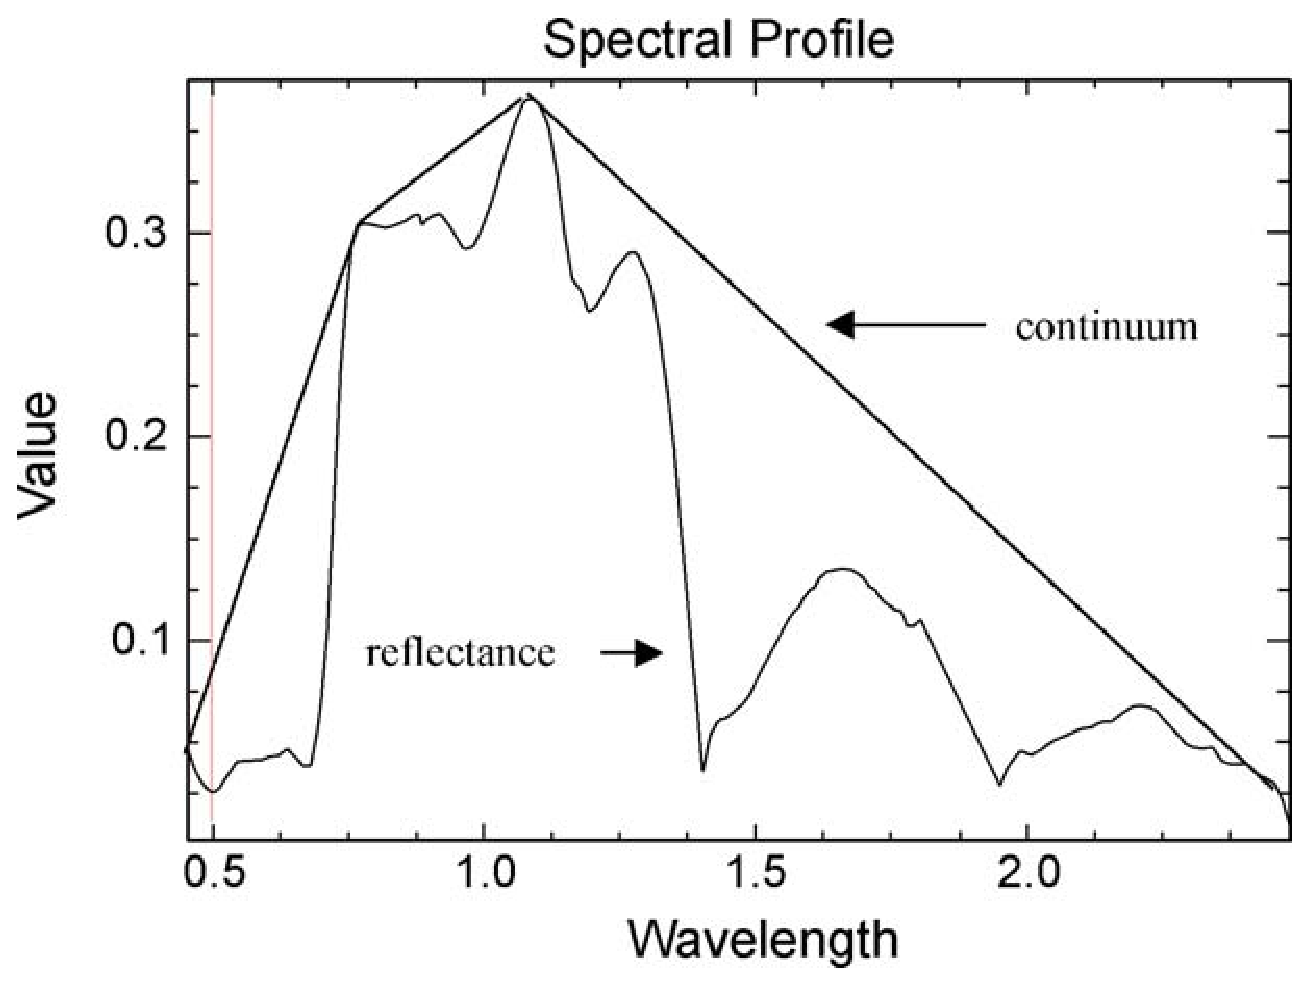
\includegraphics[width=0.5\linewidth]{./Imagenes/CR1.eps}
	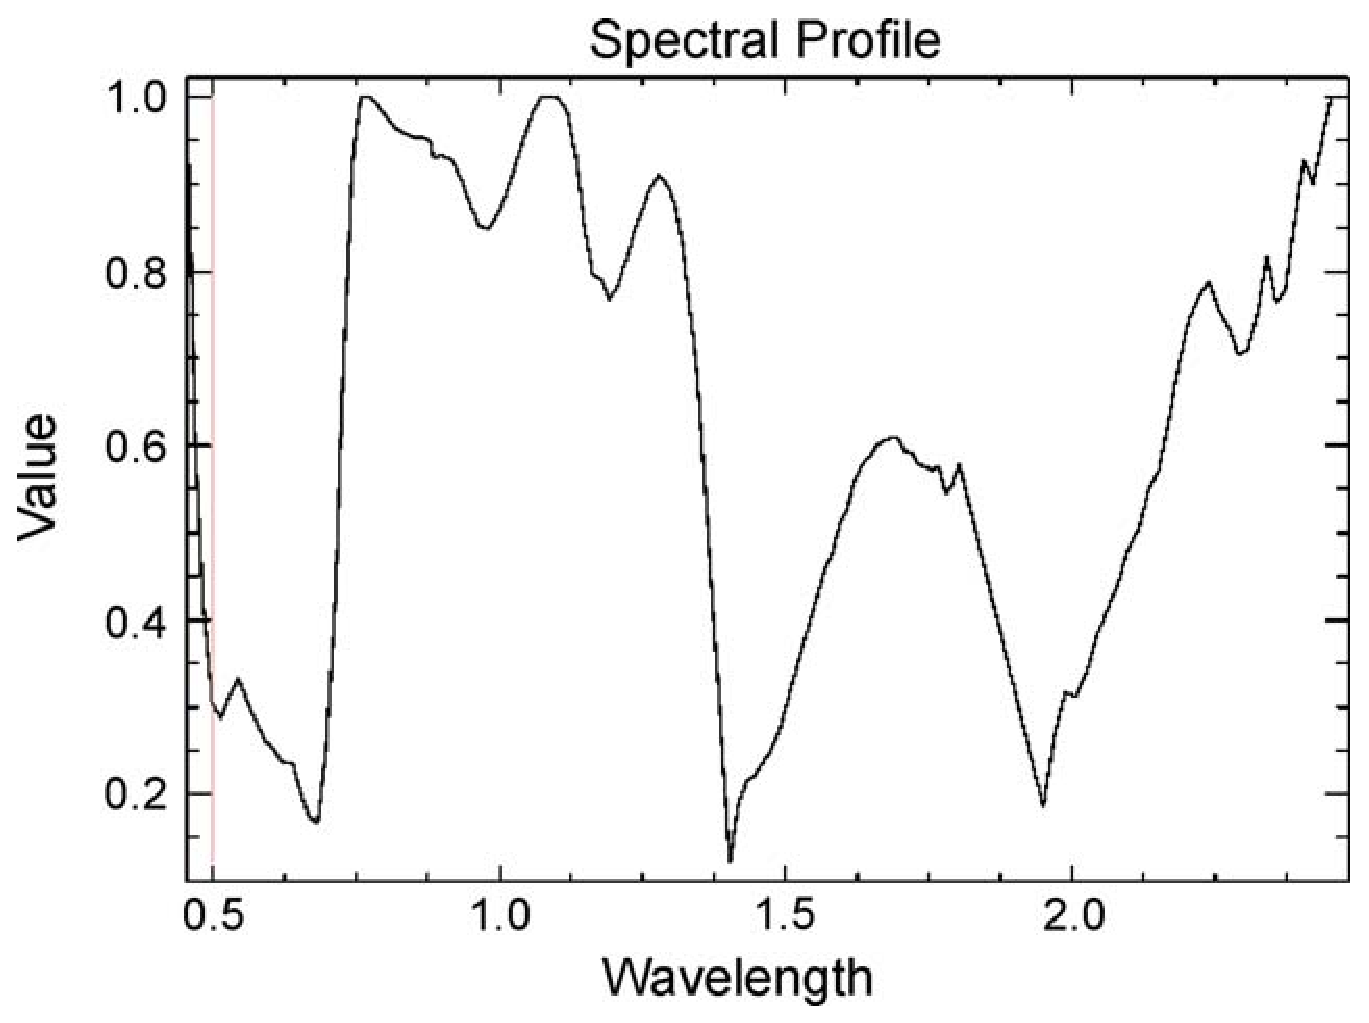
\includegraphics[width=0.5\linewidth]{./Imagenes/CR2.eps}
	\captionsetup{font={footnotesize,it}}
	\caption[Continuum Removal ejemplo]{Ejemplo de aplicación de la técnica continuum removal. Fuente:\cite{huang2004estimating}.}
	\label{fig:ejemploCR}
\end{figure}

Este método no aporta un valor numérico de cuantificación de la similitud entre dos espectros, centrándose en un análisis gráfico de cada respuesta por separado.%\Sep

El paquete base de R ya incluye las operaciones estadísticas básicas necesarias para la elaboración de la clasificación angular y el \ac{IAE} con la única excepción de que para poder aplicar el analizador \ac{CR} se debe descargar el paquete adicional \textit{prospectr} \citep{stevens2014introduction}.%\Sep

En la figura \ref{fig:CR} se muestra el script original de la función en R a la que se le aplicarán los datos de campo y que devuelve la gráfica de \ac{CR}.%\Sep

\begin{figure}
\centering
\begin{lstlisting}[language = R]
  require(prospectr) # carga del paquete necesario
  
  # aplicacion de la funcion implementada en prospectr 
  cr <- continuumRemoval(mangle1corte$V5, mangle1corte$V4,
                         type="R",
                         interpol="linear")
                         
  grafica(data1) # salida grafica a los datos iniciales
  lines(data1$V4,cr) # superposicion de la grafica de CR
\end{lstlisting}
\captionsetup{font={footnotesize,it}}
\caption[Función de \textit{Continuum Removal}]{Script de la función de \textit{Continuum Removal} en R. Elaboración propia a partir de \cite{stevens2014introduction}.}
\label{fig:CR}
\end{figure}

Se puede observar como mediante el comando inicial \textit{require()} se llama al paquete \textit{prospectr}, gracias al cual nos aseguramos que está correctamente cargado el paquete necesario para realizar las operaciones que siguen en el script \citep{stevens2014introduction}. Para ello se utilizó el instalador de paquetes de RStudio, localizando el paquete requerido en el repositorio oficial de RCRAN e instalando las dependencias necesarias, que también se podría haber hecho con el comando \textit{``install.packages()''}. El comando \textit{grafica()} es la llamada a una función creada para presentar la gráfica a nuestro gusto, mientras que con el comando \textit{lines()} se nos permite superponer la gráfica de \ac{CR} a la anterior.%\Sep

Para el correcto funcionamiento del análisis se procedió a crear una matriz de 3x481 donde las filas corresponden a las tres especies analizadas y las columnas al valor de longitud de onda. El fin es el de presentar de mejor forma los datos en la función de \ac{CR} de R y aunque el resultado es el mismo, que haciéndolo una por una, nos permite obtener este de forma más rápida y con menos pasos.%\Sep

El script original de la funcion en R previamente presentado en la figura \ref{fig:CR} sufre cambios, quedando de la siguiente manera:%\SmallSep

\begin{figure}[ht]
	\centering
	\begin{lstlisting}[language = R]
  require(prospectr)
  
  # generacion de la matriz de datos
  matriz <- matrix(c(RhizophoraCorte$V5,LagunculariaCorte$V5,
                     AvicenniaCorte$V5),
                   byrow=TRUE,
                   nrow=3,
                   ncol=481)
  
  # se especifica el numero de observaciones                 
  bandas <- mangle1corte$V4
  
  # se aplica la funcion
  cr <- continuumRemoval(matriz, bandas)
  
  # salida grafica a los datos
  matplot(bandas, t(matriz),
          type="l", ylim=c(0,1))
  matlines(bandas, t(cr2))
	\end{lstlisting}
	\captionsetup{font={footnotesize,it}}
	\caption[Función modificada de \textit{Continuum Removal}]{Script modificado de la función de \textit{Continuum Removal} escrita en R. Elaboración propia.}
	\label{fig:CRmodificado}
\end{figure}	

Donde ``manglencorte'' es el archivo de datos con el corte realizado para cada especie como se explicó anteriormente. Se crea un objeto llamado ``bandas'' tomando los valores de la fila V4 de cualquiera de los archivos de datos. Se crea la gráfica con el comandos \textit{matplot()} y con \textit{matlines()} se superpone la gráfica propia del método \ac{CR}.%\Sep

\subsection{Clasificación angular}
La clasificación angular también llamada \ac{SAM} calcula la similitud entre dos espectros a partir de su distancia angular espectral. Originalmente este método compara espectros desconocidos con otros de referencia tomados, por ejemplo, de bibliotecas espectrales o de la misma imagen \citep{girouard2004validated} con el fin de asignar píxeles desconocidos a clases de referencia conocida en una clasificación temática. El algoritmo de clasificación angular es el siguiente:

\begin{equation} \label{eq:angular}
	\theta = arcos \frac{\sum_{k=1}^{m} \rho_{i,k} \rho_{j,k}}{\sqrt{\sum_{k=1}^{m} \rho_{i,k}^{2}} \sqrt{\sum_{k=1}^{m} \rho_{j,k}^{2}}}
\end{equation}%\Sep

Siendo $\rho_{i,k}$ la reflectividad del espectro \textit{i} en una banda \textit{k}, $\rho_{j,k}$ la reflectividad del espectro \textit{j} en la misma banda y \textit{m} el número de bandas.%\Sep

Los espectros serán más similares cuanto menor sea el valor del ángulo $\theta$ de la ecuación \ref{eq:angular}.%\Sep

En la figura \ref{fig:AE} se muestra el script de la función en R a la que se le aplicarán los datos de campo y que devuelve el valor del ángulo $\theta$.

\begin{figure}
\centering
\begin{lstlisting}[language = R]
  AE <- function(i,j) {
  
    Ri = i$V5 # valores de las observaciones
    Rj = j$V5
  
  # calculo del angulo espectral para dos cubiertas
    angulo = acos (sum(Ri*Rj)/(sqrt(sum(Ri^2))*sqrt(sum(Rj^2))))
    return(angulo)
  }
\end{lstlisting}
\captionsetup{font={footnotesize,it}}
\caption[Función clasificación angular]{Función de clasificación angular en R. Elaboración propia.}
\label{fig:AE}
\end{figure}

\section{Imágenes de satélite}
\subsection{Landsat 8}\label{subsec:Landsat8}
Landsat 8 dispone de 11 bandas espectrales: 9 del sensor \ac{OLI} (expuestas en la tabla \ref{tab:sensoresOLI}) y 2 del sensor \ac{TIRS} que no son de interés para este trabajo.%\Sep

Como los datos del radiómetro de campo solo abarcan las longitudes de onda comprendidas entre $325 nm$ y $1075 nm$ solo son de interés las cinco primeras bandas que se detallan a continuación:

\begin{itemize}
	\item Banda 1 (Coastal/Aerosol) [430-450 nm]: Detecta azules y violetas intensos. Solventa los problemas de la dispersión de Rayleigh. Facilita la detección de la calidad de aguas poco profundas y partículas de polvo o aerosol en la atmósfera.
	\item Banda 2 (Blue) [450-510 nm]: Detecta el azul del espectro visible. Útil para diferenciar el suelo desnudo de la vegetación y detectar zonas pavimentadas como carreteras o áreas urbanas.
	\item Banda 3 (Green) [530-590 nm]: Detecta el verde del espectro visible. Sensible al nivel de turbidez del agua. Brillante en zonas de tierra árida y oscura en zonas boscosas o de cultivos.
	\item Banda 4 (Red) [640-670 nm]: Detecta el rojo del espectro visible. Útil en la clasificación de zonas vegetales pero no diferencia estas de agua, puesto que aparecen como zonas oscuras.
	\item Banda 5 (NIR) [850-880 nm]: Detecta el infrarrojo cercano. Especialmente importante en ecología porque la vegetación vigorosa la refleja. Útil para la obtención del \ac{NDVI} y distinguir tipos de vegetación.
\end{itemize}


\subsection{Obtención de las imágenes}
Las imágenes se obtuvieron del servicio Earth Explorer, de la \ac{EROS} de la \ac{USGS}. Estas imágenes ya vienen con una corrección geométrica previa hecha, por lo que no será necesario aplicar más correcciones de este tipo. En un archivo .txt asociado a las imágenes .tiff para cada banda se especifica que el método de corrección geométrica utilizado ha sido el de convolución cúbica.%\Sep

En concreto, los archivos que nos ofrece el servicio de descargas son:

\begin{itemize}
	\item Una imagen en composición de color natural como las que se muestran en la figura \ref{fig:imagenesLandsat}.
	\item Una imagen térmica que no nos será de utilidad.
	\item Una imagen de 8 bits que cuantifica la calidad de la observación.
	\item Las imágenes anteriormente citadas georreferenciadas.
	\item Las imágenes correspondientes a cada banda de Landsat 8 con la corrección geométrica aplicada (level 1) en formato GeoTIFF.
\end{itemize}%\Sep

Se trata de un producto de \ac{L1T} con correcciones geométricas sistemáticas aplicadas utilizando para ello puntos de control terrestre o información de posición integrada a bordo \citep{Ariza2013}. Se entrega así una imagen registrada a la proyección WGS84. Adicionalmente en este nivel de producto contiene una corrección topográfica por el desplazamiento del terreno debido al relieve. Las imágenes se encuentran en formato de \ac{ND} que se pueden transformar a valores de reflectividad \ac{TOA} en las bandas 1 a 9.%\Sep

Otra forma de obtener las imágenes de Landsat 8 es mediante el gestor de descargas Libra, que aprovecha la API del servicio de \ac{AWS} que aloja estas imágenes desde septiembre de 2014. Este nos permite elegir que bandas descargar, ahorrando tiempo en la operación.%\Sep

En cambio, para la correcta realización de este \ac{TFG} donde tenemos datos de reflectividad a nivel del suelo, necesitamos que las imágenes Landsat también muestren valores de reflectividad a ese nivel. Esto se consigue aplicando un algoritmo de corrección radiométrica a las imágenes \ac{L1T} obteniendo un producto también proporcionado por la agencia \ac{EROS} bajo demanda llamado \ac{PL8SR} \citep{USGS2015} que también se puede encontrar bajo en nombre de Landsat SR.%\Sep

Para abarcar la zona de estudio se necesitaron obtener dos imágenes que tienen las características mostradas en el cuadro \ref{tab:imagenes}. Se consideró que la diferencia temporal entre ambas imágenes y la fecha de toma de datos no era determinante suponiendo un escaso cambio fenológico de las especies de mangle en ese periodo de tiempo.%\Sep

\begin{table}[ht]
	\centering
	\begin{tabular}{@{}cccccccc@{}}
	\toprule[0.4mm]
	Imagen & Path & Row & Fecha & West & East & North & South \\
	\midrule
	1 (a) & 18 & 51 & 23/11/2014 & -89.105062 & -86.987819 & 14.067713 & 11.946409 \\
	2 (b) & 17 & 51 & 19/12/2014 & -87.549399 & -85.443030 & 14.062287 & 11.952632 \\
	\bottomrule[0.4mm]
	\end{tabular}
	\captionsetup{font={footnotesize,it}}
	\caption[Caracerísticas de las imágenes Landsat]{Características de las imágenes Landsat obtenidas de la figura \ref{fig:imagenesLandsat}. Elaboración propia.}
	\label{tab:imagenes}
\end{table}

Se observa en las imágenes de calidad de la figura \ref{fig:imagenescalidad}, en las que las nubes y nubes altas se marcan de color blanco y amarillo respectivamente, que la cobertura nubosa es aceptable para trabajar en la zona de estudio.%\Sep

\begin{figure}
	\centering
	\subfloat[Imagen Landsat path 18 row 51 (23/11/14)]{
	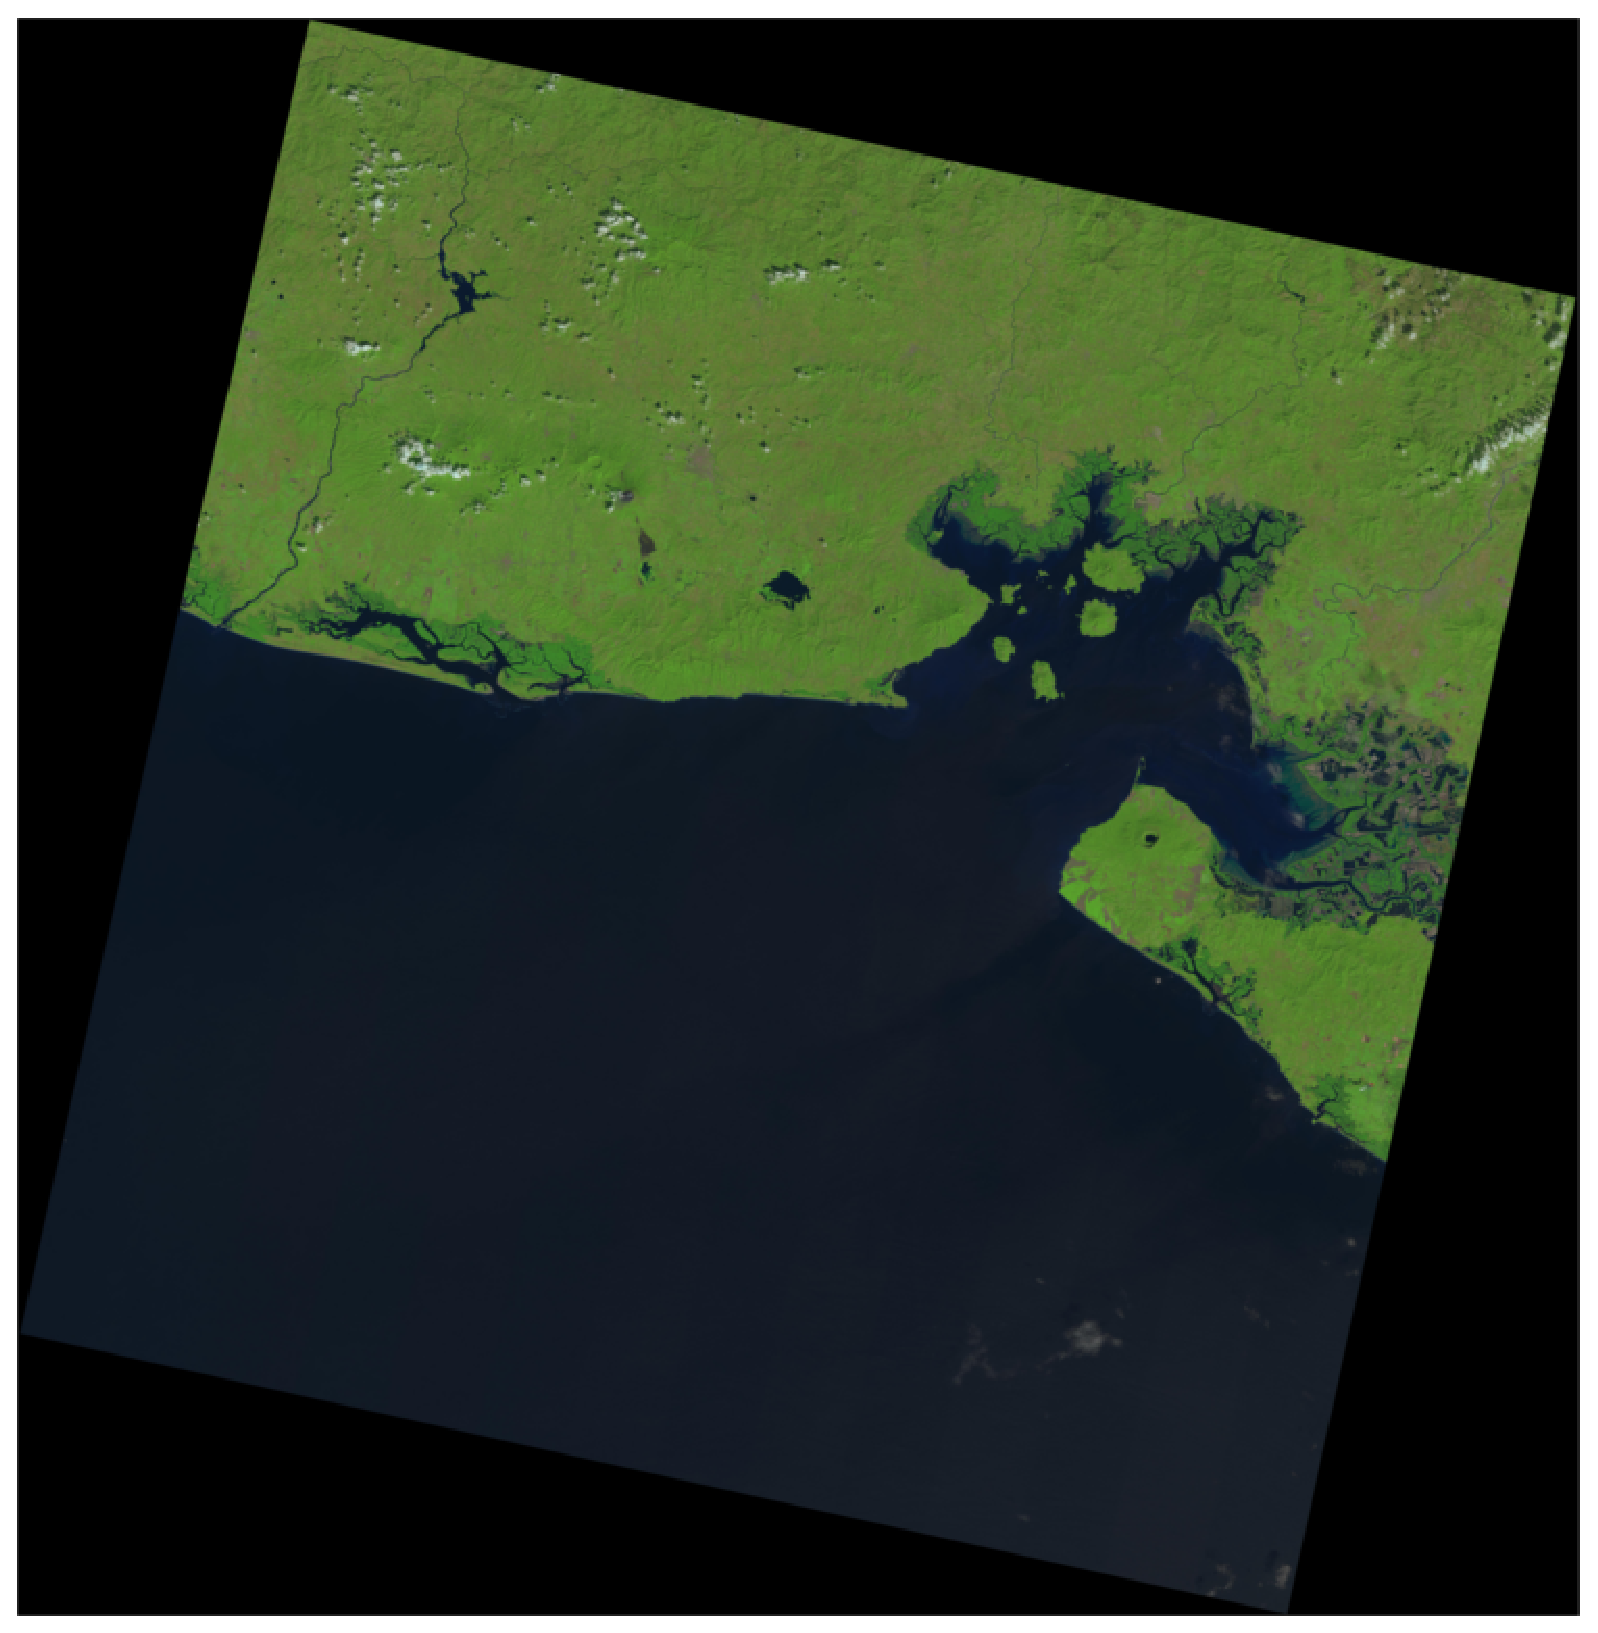
\includegraphics[width=0.45\linewidth]{./Imagenes/Landsat18.eps}}
	\subfloat[Imagen Landsat path 17 row 51 (19/12/14)]{
	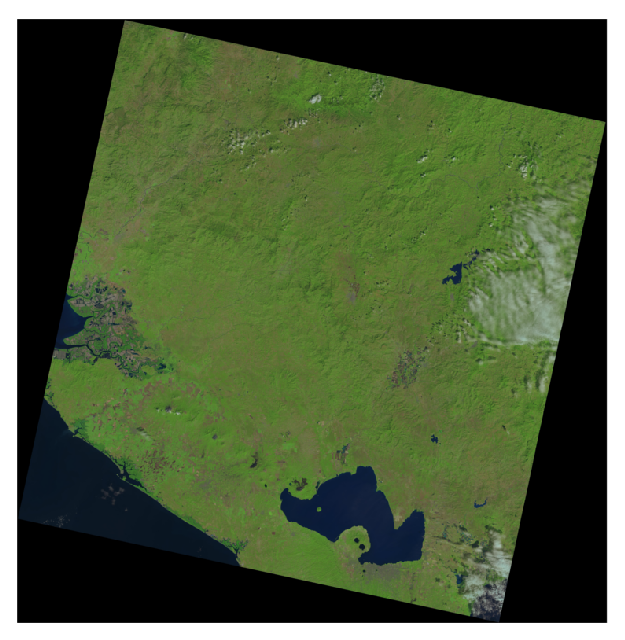
\includegraphics[width=0.45\linewidth]{./Imagenes/Landsat17.eps}}
	\captionsetup{font={footnotesize,it}}
	\caption[Imágenes Landsat]{Imágenes Landsat con corrección geométrica utilizadas para el trabajo. Fuente: USGS.}
	\label{fig:imagenesLandsat}
\end{figure}

\begin{figure}
	\centering
	\subfloat[Imagen de calidad Landsat path 18 row 51 (06/10/14)]{
	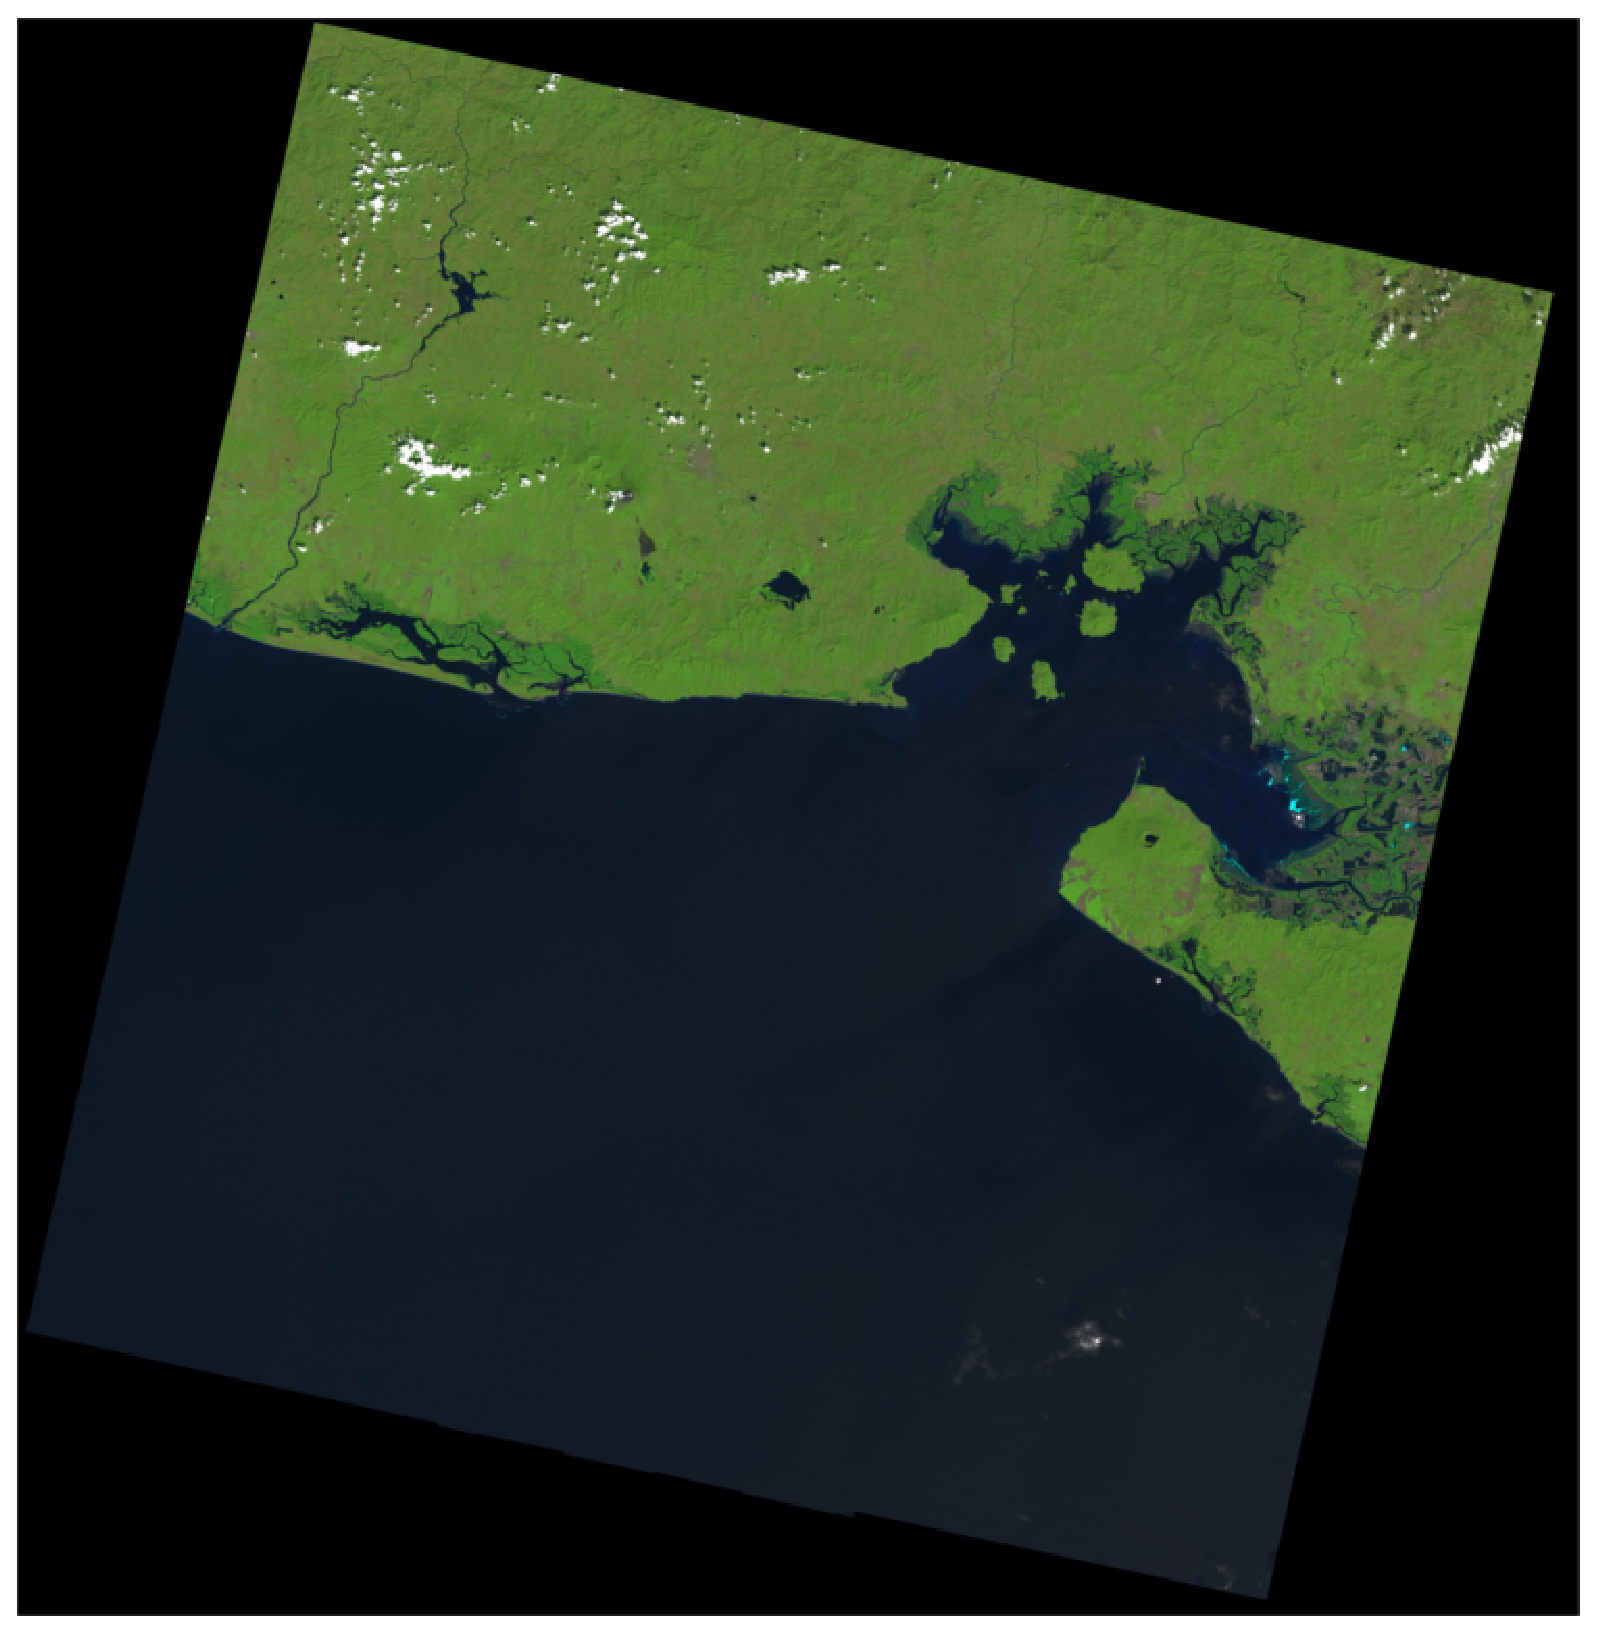
\includegraphics[width=0.45\linewidth]{./Imagenes/LandsatQ18.eps}}
	\subfloat[Imagen de calidad Landsat path 17 row 51 (16/11/14)]{
	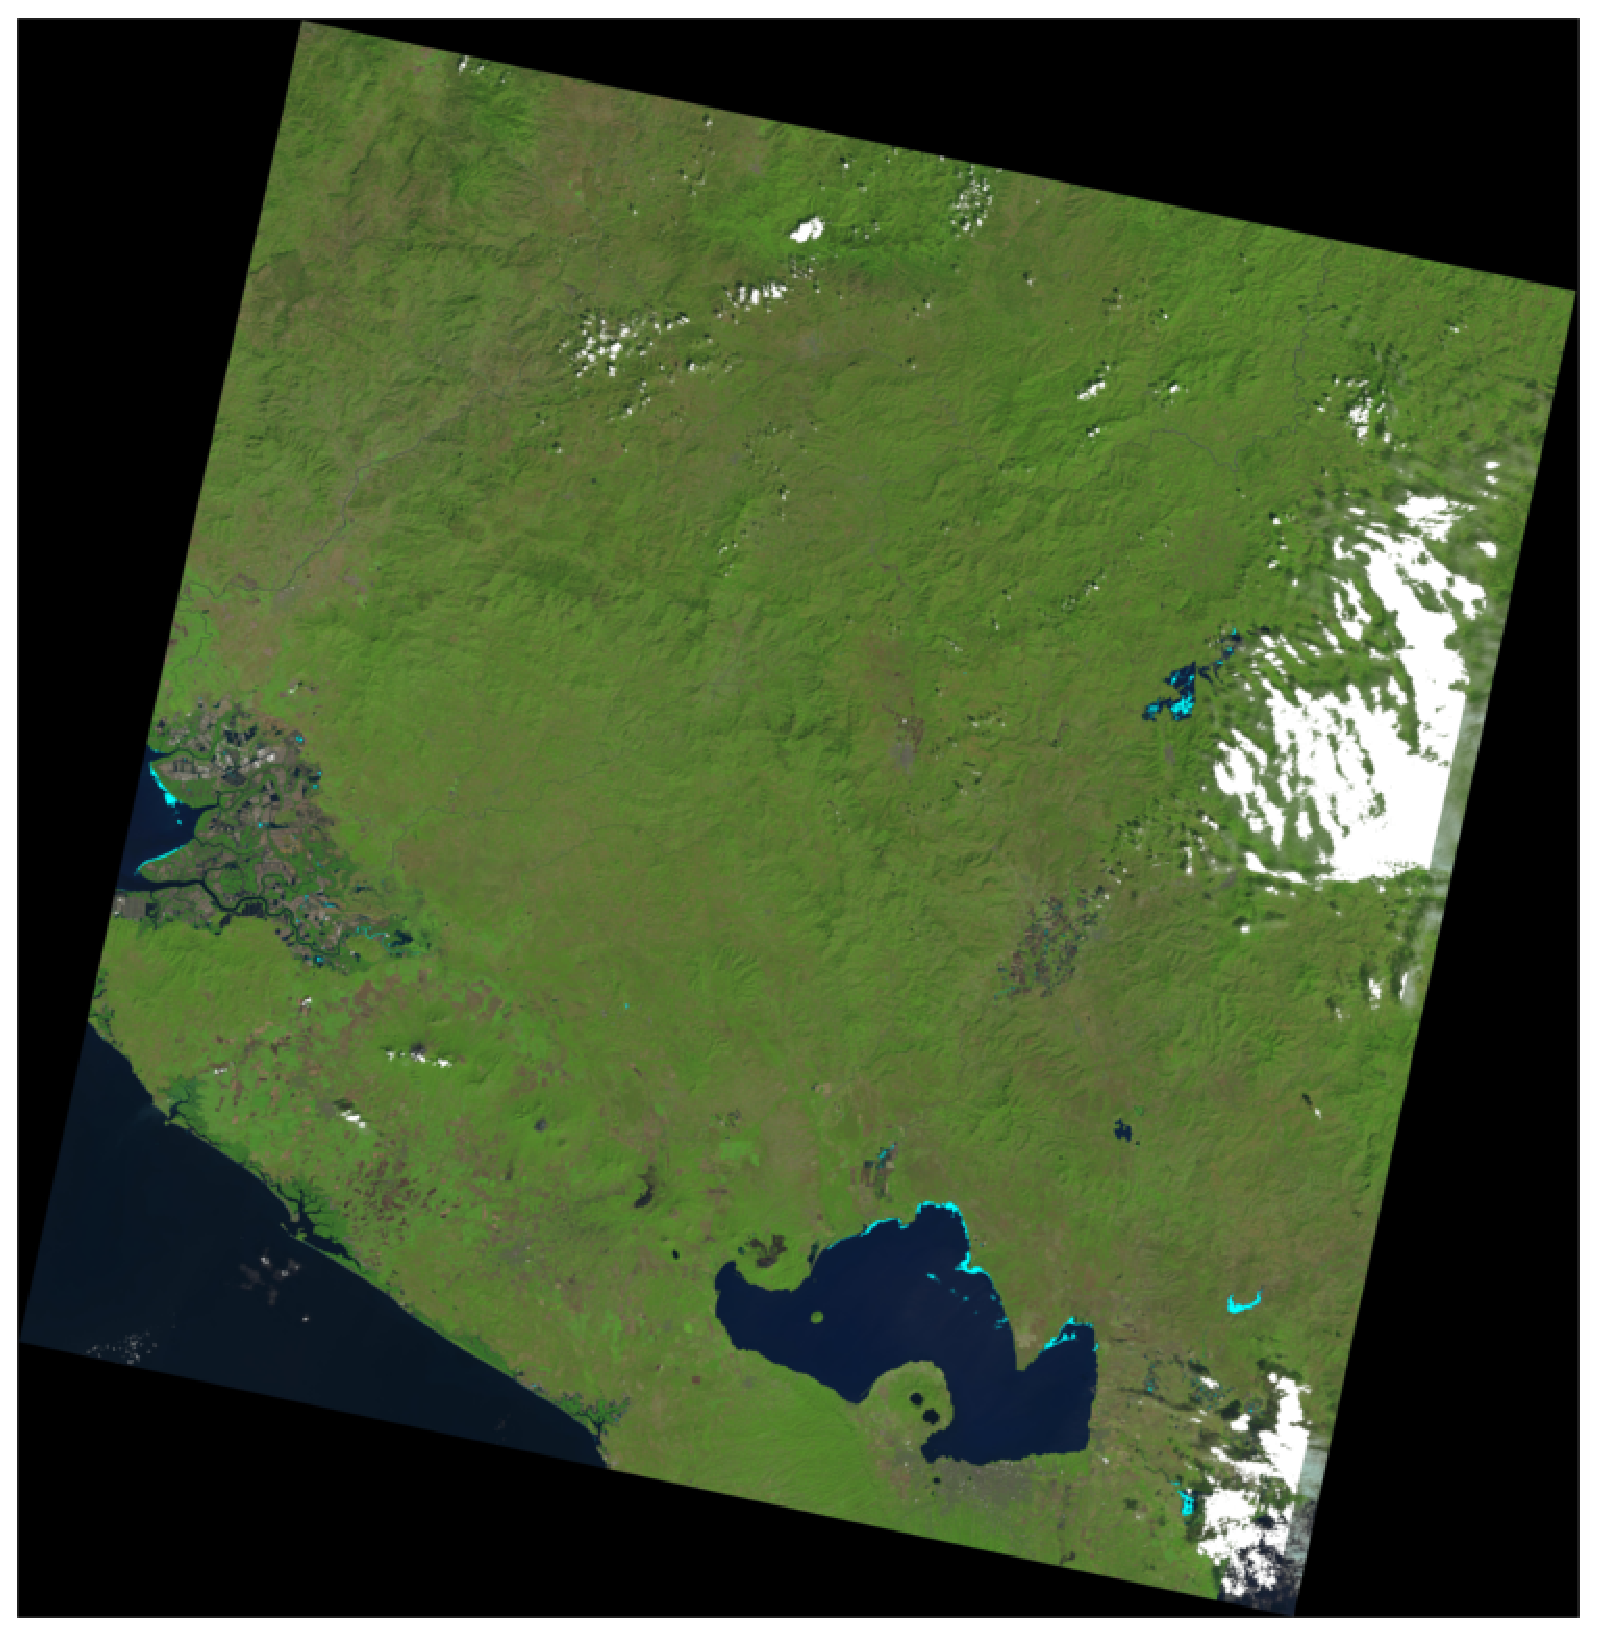
\includegraphics[width=0.45\linewidth]{./Imagenes/LandsatQ17.eps}}
	\captionsetup{font={footnotesize,it}}
	\caption[Imágenes de calidad de Landsat]{Imágenes de calidad de Landsat de 8 bits. Fuente: USGS.}
	\label{fig:imagenescalidad}
\end{figure}

Las imágenes utilizan el siguiente código de identificación en el nombre \citep{Ariza2013} \citep{USGS2015}:

\begin{center}
	\fbox{LXSPPPRRRYYYYDDDGSIVV}
\end{center}

\noindent donde:

\begin{itemize}
	\item L: Landsat.
	\item X: Sensor.
	\item S: Satélite.
	\item PPP: Path.
	\item RRR: Row.
	\item YYYY: Año de adquisición de la imagen.
	\item DDD: Día juliano del año.
	\item GSI: Identificador de la estación terrestre de seguimiento.
	\item VV: Versión del archivo.
\end{itemize}

\subsection{Tratamientos previos}
Como se decía en el apartado anterior, la geometría de las imágenes ya está corregida. Pero es necesario realizar algunos procedimientos antes de unirlas y recortarlas finalmente para que se adapten a la zona de estudio y sea más cómodo trabajar con ellas. Estos procedimientos son el tratamiento de los valores nulos, la transformación de los \ac{ND} en reflectancias, el mosaico de imágenes, su posterior recorte y la aplicación de un filtro de paso bajo.%\Sep

Lo primero que se debe hacer en GRASS es crear la localización \textit{(location)} de nuestro proyecto y añadir las imágenes al directorio de mapas \textit{(mapset)}. Los datos de la localización se establecen gracias a la lectura por parte de GRASS de la configuración de proyección y datum de un archivo de datos georreferenciado, es decir, de cualquier imagen de Landsat del trabajo. Las imágenes se añadirán al \textit{mapset} con el comando \textit{r.in.gdal}.

\subsubsection{Valores nulos}
El tratamiento de los valores nulos se lleva a cabo mediante el comando \textit{r.null} como sigue:

\begin{figure}[ht]
\centering
\begin{boxedverbatim}
	r.null map=LC80180512014279LGN00_B1@TFG setnull=0 null=-9999
\end{boxedverbatim}
\captionsetup{font={footnotesize,it}}
\caption[Valores nulos]{Tratamiento de valores nulos en GRASS con el comando \textit{r.null}.}
\end{figure}

\noindent donde \textit{``map''} corresponde a la banda a tratar seguido por el \textit{mapset}, \textit{``setnull''} indica el valor de los elementos nulos y \textit{``null''} indica el nuevo valor de estos elementos. Se elige un valor de -9999 para evitar posibles errores de realizarse, por ejemplo un \ac{NDVI} que trabaja con valores de píxel de [-1,1].%\Sep

Este no es un procedimiento obligatorio aunque recomendable ya que los geoprocesos aplicados siguientes, como el mosaico de imágenes, ya implican un tratamiento de valores nulos.

%\subsubsection{Transformación a reflectancias}
%Los \ac{ND} pueden ser reescalados a valores de reflectancias \ac{TOA} gracias a los coeficientes radiométricos provistos en el archivo .txt que acompaña a las imágenes. Esta transformación se hará con el comando \textit{i.landsat.toar} como sigue:

%\begin{figure}[ht]
%\centering
%\begin{boxedverbatim}
%	i.landsat.toar
%	input_prefix=LC80170512014320LGN00_B
%	output_prefix=LC80170512014320LGN00_TOAR_B
%	metfile=/home/marcos/grassdata/Imagenes/Landsat/
%	P17R51/Base/LC80170512014320LGN00_MTL.txt
%	sensor=oli8
%	method=dos4
%	date=2014-11-16
%	sun_elevation=52.01756824
%\end{boxedverbatim}
%\captionsetup{font={footnotesize,it}}
%\caption[Transformación a reflectancias]{Transformación a reflectancias TOA en GRASS con el comando \textit{i.landsat.toar}.}
%\end{figure}

%\noindent donde \textit{``input\_prefix''} es el prefijo del nombre de las imágenes para cada banda, \textit{``output\_prefix''} es el prefijo que le queremos dar a las nuevas imágenes corregidas, \textit{``metfile''} es el archivo de metadatos asociado, \textit{``sensor''} el tipo de sensor, \textit{``date''} es la fechas de adquisición y \textit{``sun\_elevation''} la elevación en grados del Sol.

\subsubsection{Mosaico de imágenes}
Para realizar el mosaico de las dos imágenes de las que disponemos tenemos dos opciones: utilizando la herramienta \textit{gdal\_merge.py} y hacerlo en GRASS. Para utilizar la herramienta de la librería \ac{GDAL} gdal\_merge.py debemos tener las siguientes consideraciones previas:

\begin{itemize}
	\item Es un método que se ejecuta en la terminal de Linux. Para un método guiado se utilizaría, por ejemplo, la herramienta \textit{raster/combinar} en QGIS o el método de GRASS que se expondrá más adelante.
	\item Las dos imágenes deben estar en el mismo sistema de coordenadas.
	\item Utiliza como método de remuestreo el de vecino más próximo.
	\item La última imagen de la lista será copiada sobre la precedente en el caso de haber solape.
\end{itemize}

La línea de comando en cuestión es la siguiente (para las imágenes de la primera banda y en el caso de tener situadas las imágenes en la misma carpeta):

\begin{figure}[ht]
\centering
\begin{boxedverbatim}
	gdal_merge.py -n 0 -v LC80170512014320LGN00_B1.TIF 
	LC80180512014279LGN00_B1.TIF -o mosaico1.tif
\end{boxedverbatim}
\captionsetup{font={footnotesize,it}}
\caption[Mosaico de imágenes]{Mosaico de imágenes con herramientas GDAL.}
\end{figure}

En este caso se utilizan los comandos asociados u opciones siguientes: -n para que se ignoren los píxeles con valores nulos, -v para que se detallen las operaciones realizadas y -o que permite dar nombre al archivo de salida. Con este método no sería necesario realizar el tratamiento de valores nulos.%\Sep

En la figura \ref{fig:dialogomosaico} se observa el diálogo resultante de la operación anterior que confirma que se ha hecho bien el mosaico. En el tenemos datos de las imágenes como el nombre, las coordenadas de la esquina superior izquierda e inferior derecha, tamaño del píxel y tiempo que se necesitó para realizar la operación.%\Sep

\begin{figure}
	\centering
	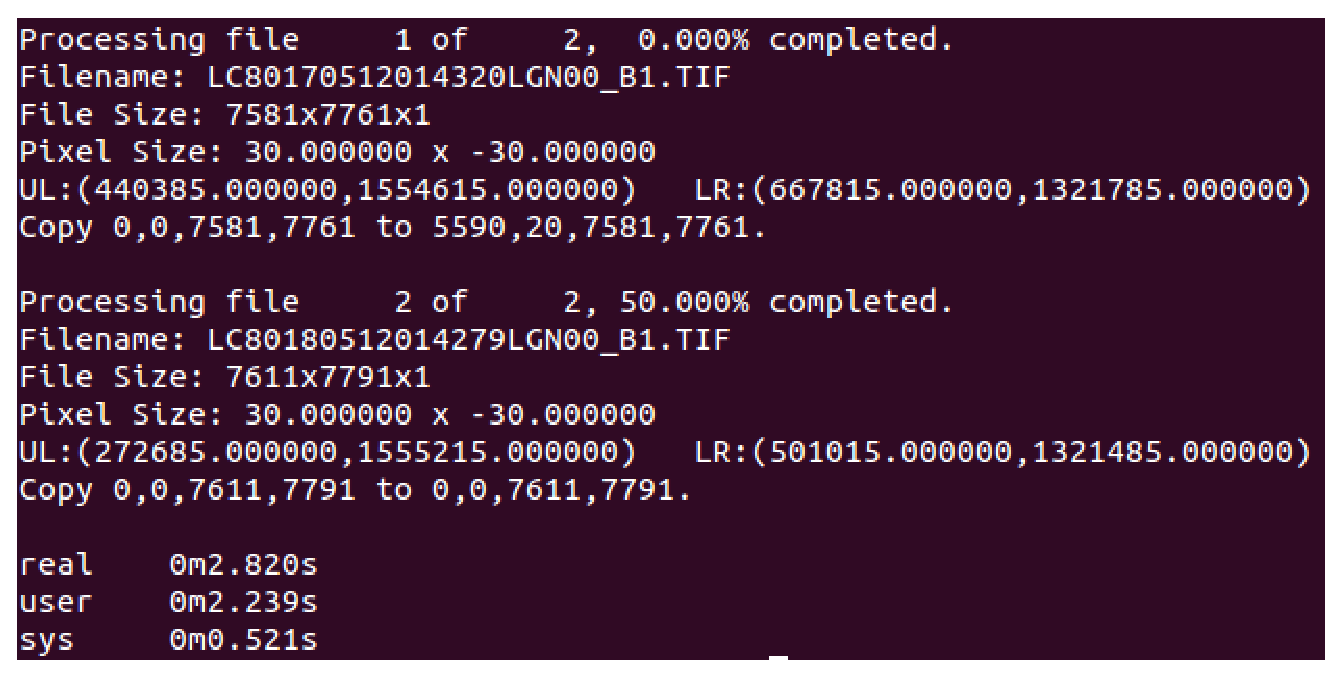
\includegraphics[width=0.8\linewidth]{./Imagenes/Dialogo_mosaico.eps}
	\captionsetup{font={footnotesize,it}}
	\caption[Diálogo del mosaicado]{Diálogo resultante del mosaicado de las imágenes en la terminal de Linux. Elaboración propia.}
	\label{fig:dialogomosaico}
\end{figure}

De hacerlo en GRASS, el comando sería \textit{r.patch}, con la salvedad de que las dos imágenes deben estar en la misma región de cálculo, la cual se puede ver en el cuadro \ref{tab:region}, quedando la línea de orden de la figura \ref{fig:rpatch}.

\begin{figure}[ht]
\centering
\begin{boxedverbatim}
	r.patch input=LC80180512014327LGN00_sr_band1@TFG,
	              LC80170512014352LGN00_sr_band1@TFG 
	output=Mosaico_B1
\end{boxedverbatim}
\captionsetup{font={footnotesize,it}}
\caption[Mosaico de imágenes en GRASS]{Mosaico de imágenes en GRASS mediante el comando \textit{r.patch}.}
\label{fig:rpatch}
\end{figure}

\subsubsection{Recorte de la imagen}
Para trabajar solamente con la zona de estudio es necesario recortar la imagen o reducir la región de cálculo. Para ello empleamos las opciones de visualización de GRASS con una extensión de coordenadas superior derecha de (516000 , 1501230) e inferior izquierda de (377940 , 1412100) como se muestra en el cuadro \ref{tab:region}. Una vez fijada se selecciona la opción de zoom ``set computational region from display extent'' que simplemente reduce la región de cálculo previamente establecida a la extensión de la visualización actual y nos permite realizar operaciones en esta.%\Sep

\begin{table}[ht]
	\centering
	\begin{tabular}{@{}rcc@{}}
	\toprule[0.4mm]
	& Extensión original & Extensión reducida\\
	\midrule
	Proyección & 1 (UTM) & 1 (UTM) \\
	Zona & 16 & 16 \\
	Datum & WGS84 & WGS84 \\
	Elipsoide & WGS84 & WGS84 \\
	Norte & 1555215 &1501230 \\
	Sur & 1321485 & 1412100 \\
	Oeste & 272685 & 377940 \\
	Este & 667815 & 516000 \\
	Res. esp. vertical (m) & 30 & 30 \\
	Res. esp. horizontal (m) & 30 & 30\\
	Filas & 7791 & 2971 \\
	Columnas & 13171 & 4602 \\
	Celdas & 102615261 & 13672542 \\
	\bottomrule[0.4mm]
	\end{tabular}
	\captionsetup{font={footnotesize,it}}
	\caption[Datos de las regiónes de trabajo]{Datos de las regiónes de trabajo establecidas en GRASS.}
	\label{tab:region}
\end{table}

Con el comando \textit{r.resample} se hace el remuestreo mediante vecino más próximo del área del recorte permitiendo obtener la imagen final para cada banda. El comando se emplea de la siguiente forma para cada banda:

\begin{figure}[ht]
\centering
\begin{boxedverbatim}
	r.resample input=MosaicoB1@TFG output=L8GF_SRB1
\end{boxedverbatim}
\captionsetup{font={footnotesize,it}}
\caption[Recorte de la imagen]{Recorte de la imagen en GRASS con el comando \textit{r.resample}.}
\end{figure}

A la hora de nombrar la imagen resultante en el \textit{output} ya se busca un código que identifique fácilmente la imagen. En este caso L8GF quiere decir que se trata de una imagen Landsat 8 del Golfo de Fonseca exclusivamente, mientras que SRB1 quiere decir que se trata de una imagen con reflectividades a nivel de suelo de la banda 1.

\subsubsection{Filtro de paso bajo}
La aplicación de un filtro de media a la imagen Landsat de la zona de estudio permite eliminar ruido y disminuir contrastes \citep{aldalur2002}. Antes de aplicar el filtro conviene realizar una copia de seguridad de la imagen debido a que se van a modificar los valores de reflectividad originales. Para ello se emplea el comando \textit{r.out.gdal} que permite exportar las imágenes a formato GeoTIFF.%\Sep

Se aplica a la imagen la siguiente función en cada píxel:

\begin{equation}
	g(x,y)=\frac{1}{9} \cdot \left(\begin{array}{ccc}
								   	1&1&1\\
								   	1&1&1\\
							 	   	1&1&1
								   \end{array}
							 \right)
\end{equation}
\noindent donde $g(x,y)$ es el nuevo valor del píxel localizado en las coordenadas \textit{x} e \textit{y} de la imagen y la matriz refleja la dimensión 3x3 del filtro, afectando así a $g(x,y)$ solamente los valores de los píxeles vecinos.%\Sep

La operación es realizada en GRASS mediante el comando \textit{r.neighbors} como sigue:

\begin{figure}[ht]
\centering
\begin{boxedverbatim}
	r.neighbors input=L8GF_SRB1@TFG output=L8GF_SRFB1 size=3
\end{boxedverbatim}
\captionsetup{font={footnotesize,it}}
\caption[Filtro de paso bajo]{Filtro de paso bajo en GRASS con el comando \textit{r.neighbors}.}
\end{figure}

El comando admite varias operaciones de filtrado como entre otras: media, mediana y moda. Al no especificar ninguna opción extra en el comando más que el tamaño de matriz de filtrado que se aplica, GRASS aplica el método de media por defecto. En el código de nombre de la imagen se va a añadir una F para indicar que las imágenes están filtradas.

El resultado de estos tratamientos se puede ver en las figuras \ref{fig:gf432} y \ref{fig:gf543}.
\begin{figure}
	\centering
	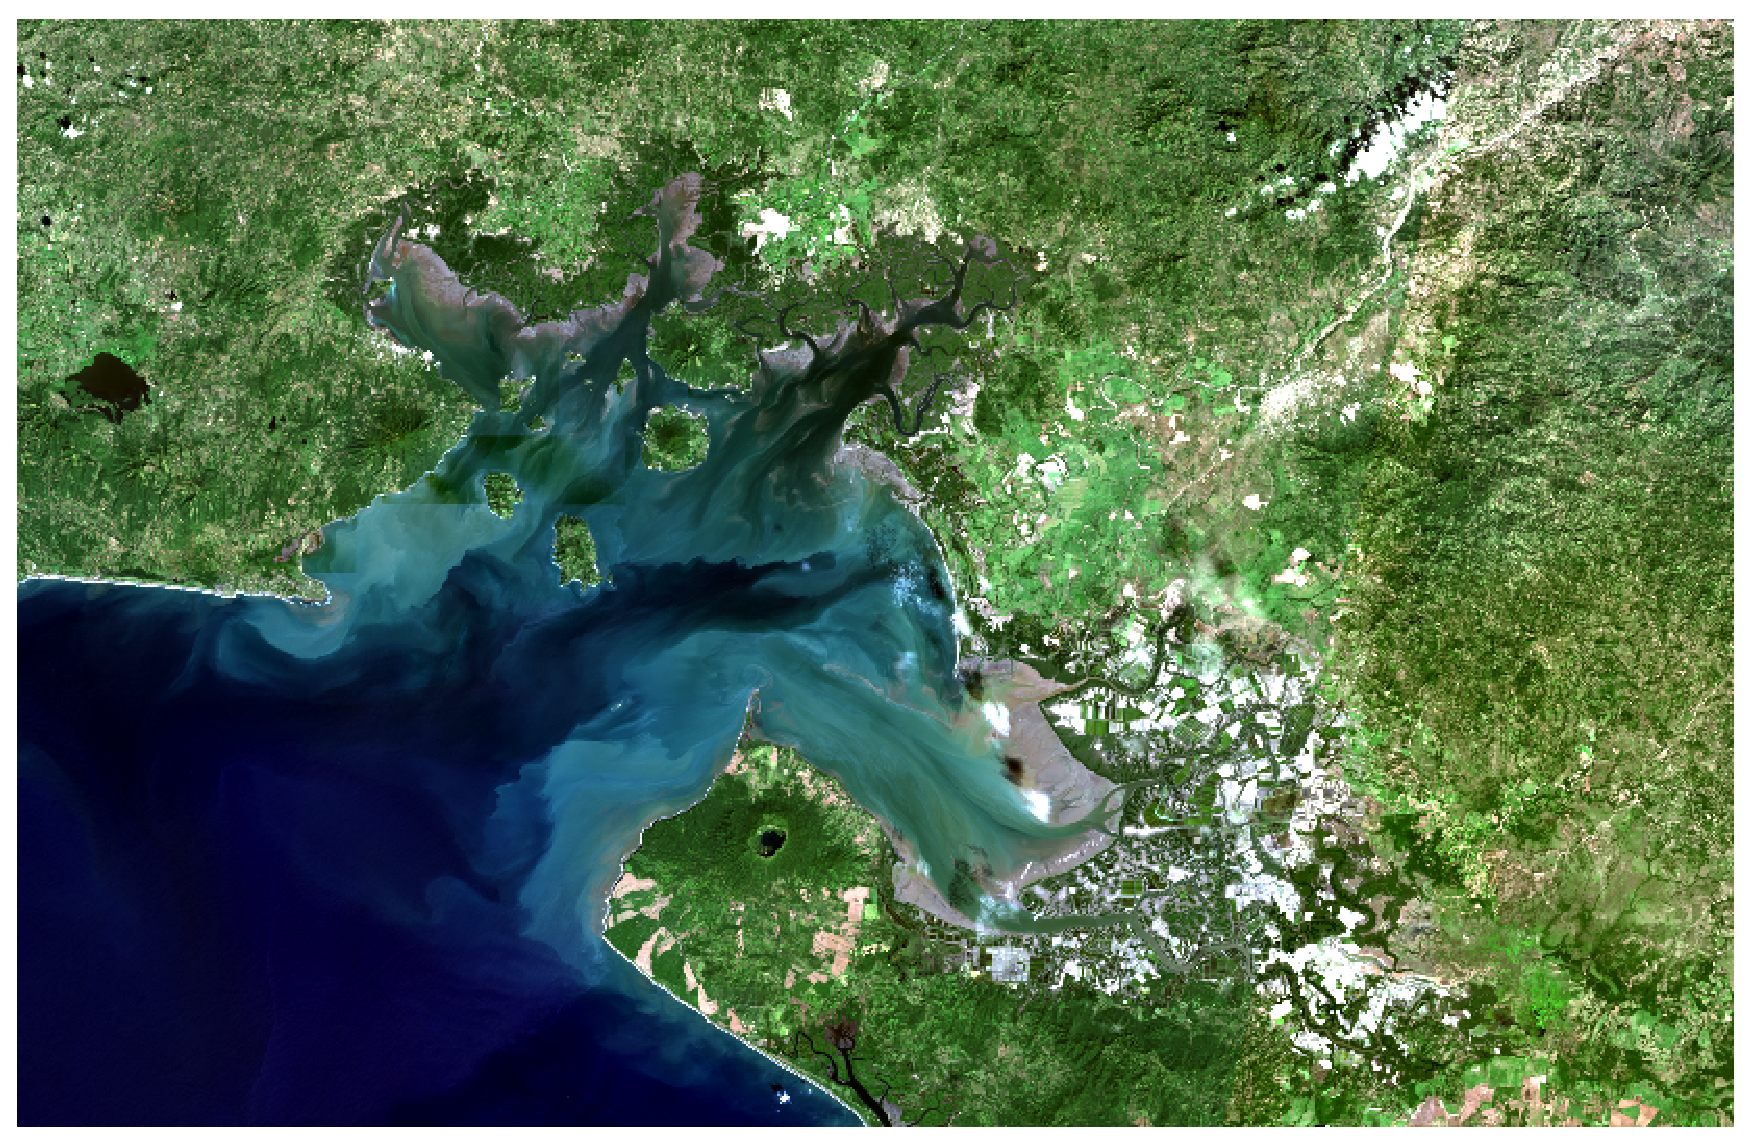
\includegraphics[width=0.9\linewidth]{./Imagenes/GF432.eps}
	\captionsetup{font={footnotesize,it}}
	\caption[Composición en color real]{Resultado de la imagen en una composición de color real (4-3-2). Imagen exportada de GRASS. Elaboración propia.}
	\label{fig:gf432}
\end{figure}

\begin{figure}
	\centering
	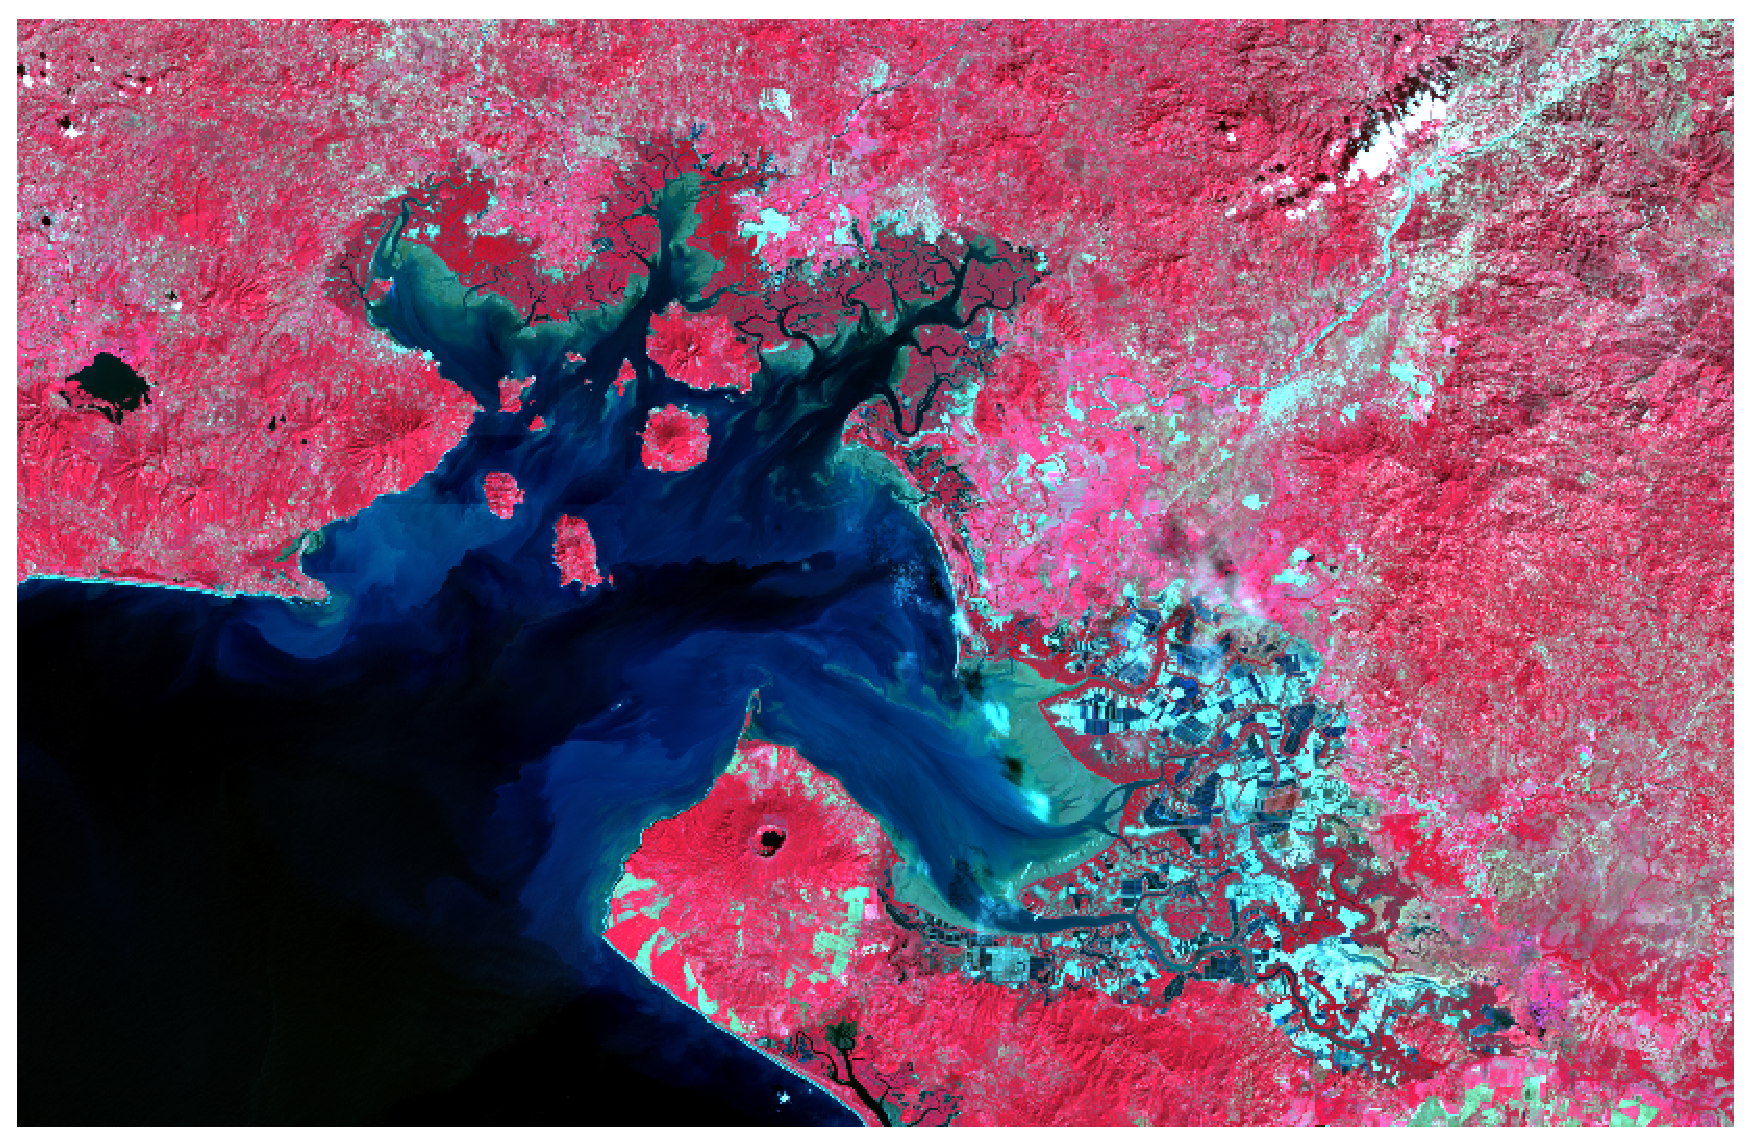
\includegraphics[width=0.9\linewidth]{./Imagenes/GF543.eps}
	\captionsetup{font={footnotesize,it}}
	\caption[Composición en falso color]{Resultado de la imagen en una composición de falso color (5-4-3). Imagen exportada de GRASS. Elaboración propia.}
	\label{fig:gf543}
\end{figure}

\section{Comprobación}
Debemos saber si los datos de reflectividad de las especies de mangle se adaptan a los datos de las imágenes raster de Landsat 8 que se han corregido. Para ello tomamos la serie de puntos en los que se conoce la existencia de bosque de mangle (cuadro \ref{tab:puntos}). Se creará en GRASS una capa vectorial con estos puntos a las que se le añadirán los valores raster de reflectividad de cada banda. Los pasos a seguir fueron los siguientes:

\begin{itemize}
	\item Creación de una capa vectorial en blanco de nombre ``puntos'' y añadirla al árbol de capas. En esta capa se digitalizarán un total de 10 puntos en los que se supone la existencia de bosque de mangle.
	\item Crear una base de datos asociada a la capa con \textit{v.db.addtable} asignando nuevos campos: ``x'' e ``y'' de tipo ``double'' que se actualizarán con las coordenadas de los puntos. También se añadirán a la tabla columnas para alojar el valor de los datos de cada una de las bandas en cada punto nombradas como B1, B2, B3, B4 y B5 de tipo ``double''.
	\item Actualización de los campos de coordenadas mediante el comando \textit{v.to.db} como se muestra en la figura \ref{fig:v.to.db} donde \textit{map} designa el vectorial que tiene la tabla asociada, \textit{option} indica que queremos actualizar coordenadas y \textit{columns} son los nombres de las columnas de coordenadas de nuestra tabla.
	
\begin{figure}[ht]
\centering
\begin{boxedverbatim}
	v.to.db map=puntos@TFG option=coor columns=x,y
\end{boxedverbatim}
\captionsetup{font={footnotesize,it}}
\caption[Actualización de coordenadas]{Actualización del campo coordenadas en GRASS con el comando \textit{v.to.db}.}
\label{fig:v.to.db}
\end{figure}	
	
	\item Actualización de los campos de datos del raster mediante el comando \textit{v.what.rast} como se muestra en la figura \ref{fig:v.what.rast} donde \textit{vector} indica cual es el vectorial que deseamos actualizar, \textit{raster} es el raster del que se tomarán los datos y \textit{column} el nombre del campo a actualizar.
\end{itemize}

\begin{figure}[ht]
\centering
\begin{boxedverbatim}
	v.what.rast vector=puntos@TFG raster=L8GF_SRFB1@TFG column=B1
\end{boxedverbatim}
\captionsetup{font={footnotesize,it}}
\caption[Actualización de los datos raster]{Actualización de los campos de datos raster en GRASS con el comando \textit{v.what.rast}.}
\label{fig:v.what.rast}
\end{figure}

\section{Clasificación de imágenes}
Con las figuras \ref{fig:gf432} y \ref{fig:gf543} del apartado anterior, composiciones en color real y falso color respectivamente, se puede observar como efectivamente el bosque de mangle se sitúa a lo largo de toda la costa del golfo adentrándose unos kilómetros al interior. Lo que se busca con la clasificación es reafirmar este hecho así como detectar de forma más clara esas zonas donde la proliferación de estanques de cría de camarón y salineras están afectando al ecosistema del manglar.%\Sep

Puesto que los datos disponibles no permiten la aplicación de un clasificador como el de paralelepípedos, ideal para utilizar valores estadísticos extraídos del análisis de datos, se procedió a emplear el \ac{MLC} para una clasificación supervisada y no supervisada y el clasificador \ac{SAM} para una segunda clasificación no supervisada. Debido a esto se incluyeron en el grupo de imágenes las correspondientes a las bandas 6 y 7 de Landsat 8 que servirán para refinar la clasificación. Un paso previo a la clasificación es la creación de un grupo y subgrupo de imágenes con el comando \textit{i.group} que en este caso reciben el mismo nombre: L8GF.%\Sep

Para la primera clasificación no supervisada se empleó inicialmente el comando \textit{i.cluster} (figura \ref{fig:cluster}) para crear la agrupación o \textit{cluster} de entrada con las firmas resultantes y posteriormente se aplicó el clasificador \ac{MLC} con \textit{i.maxlik} (figura \ref{fig:maxlik}). Donde una vez especificado el grupo y subgrupo de las imágenes se debe dar nombre al archivo de firmas y el número de clases. Se decidió utilizar solamente 6 clases dado que lo realmente importante para el trabajo es definir esas zonas donde existe cobertura de mangle y un mayor número daría lugar a confusión y la necesidad de realizar una reclasificación para reducir el número de clases.%\Sep

\begin{figure}[ht]
	\centering
	\begin{boxedverbatim}
	i.cluster group=L8GF@TFG subgroup=L8GF
	signaturefile=firmas1 classes=6
	\end{boxedverbatim}
	\captionsetup{font={footnotesize,it}}
	\caption[Generación de firmas \textit{i.cluster}]{Generación de firmas para la clasificación no supervisada con \textit{i.cluster}.}
	\label{fig:cluster}
\end{figure}

\begin{figure}[ht]
	\centering
	\begin{boxedverbatim}
	i.maxlik group=L8GF@TFG subgroup=L8GF
	signaturefile=firmas1 output=clasnosup
	\end{boxedverbatim}
	\captionsetup{font={footnotesize,it}}
	\caption[Clasificación con \textit{i.maxlik}]{Aplicación del clasificador \ac{MLC} con \textit{i.maxlik}.}
	\label{fig:maxlik}
\end{figure}

Para la clasificación supervisada se necesita crear una serie de áreas de entrenamiento primero como capa vectorial para posteriormente transformarla a capa ráster (detalle en figura \ref{fig:detalle_training}) con el fin de agrupar los píxeles cuyo valor servirá ara generar el archivo de firmas con el comando \textit{i.gensigset} de forma similar a \textit{i.cluster}. Previamente debemos crear en la base de datos asociada a la capa de entrenamiento dos nuevas categorías obligatorias referentes al número de categoría y nombre y una opcional referente a la tabla de color que se tomará para realizar el mapa (cuadro \ref{tab:tabla_training}). Al hacer la transformación se debe especificar cada una de estas categorías en el comando \textit{v.to.rast} como se muestra en la figura \ref{fig:conversion}.%\Sep

\begin{figure}
	\centering
	\includegraphics[width=0.9\linewidth]{./Imagenes/Detalle_training.eps}
	\captionsetup{font={footnotesize,it}}
	\caption[Detalle de áreas de entrenamiento]{Detalle de las áreas de entrenamiento tomadas sobre imagen en falso color. Imagen exportada de GRASS.}
	\label{fig:detalle_training}
\end{figure}

\begin{figure}
	\centering
	\begin{boxedverbatim}
	v.to.rast input=vtraining@TFG output=rtraining
	use=attr attribute_column=cat
	rgb_column=color label_column=class
	\end{boxedverbatim}
	\captionsetup{font={footnotesize,it}}
	\caption[Conversión vectorial a ráster]{Conversión de capa vectorial a ráster de las áreas de entrenamiento con el comando \textit{v.to.rast}.}
	\label{fig:conversion}
\end{figure}

\begin{table}[ht]
	\centering
	\begin{tabular}{@{}cccc@{}}
	\toprule[0.4mm]
	cat & class & color & n\_cells\\
	\midrule
	1 & Mangle & 0:128:0 & 4139\\
	2 & Estero & 139:105:20 & 3789\\
	3 & Agricultura & 255:255:0 & 6784\\
	4 & Estanque & 173:216:230 & 3139\\
	5 & Vegetacion & 144:238:144 & 3246\\
	\bottomrule[0.4mm]
	\end{tabular}
	\captionsetup{font={footnotesize,it}}
	\caption[Base de datos de áreas de entrenamiento]{Base de datos asociada a la capa vectorial de áreas de entrenamiento. Elaboración propia.}
	\label{tab:tabla_training}
\end{table}

Para realizar la clasificación aplicando el \ac{SAM} se recurrió a un script en R con la función del algoritmo implementada \ref{fig:R_SAM}. Para el correcto funcionamiento del script se necesita tener instalado y funcionando los paquetes oficiales \textit{raster}, \textit{rgdal} y \textit{sp} con el fin de que R permita la carga de archivos raster tipo \ac{TIFF} y hacer operaciones con ellos.

\begin{figure}
\begin{lstlisting}[language = R]
  require(rgdal)
  require(raster)

  # Carga de imagenes Landsat. Bandas 1-7
  b1 <- raster("/home/marcos/TrabajoFinGrado//L8GF_B1.TIFF")
  b2 <- raster("/home/marcos/TrabajoFinGrado//L8GF_B2.TIFF")
  b3 <- raster("/home/marcos/TrabajoFinGrado//L8GF_B3.TIFF")
  b4 <- raster("/home/marcos/TrabajoFinGrado//L8GF_B4.TIFF")
  b5 <- raster("/home/marcos/TrabajoFinGrado//L8GF_B5.TIFF")
  b6 <- raster("/home/marcos/TrabajoFinGrado//L8GF_B6.TIFF")
  b7 <- raster("/home/marcos/TrabajoFinGrado//L8GF_B7.TIFF")

  # Agrupamiento en un stack
  imagen  <- stack(b1,b2,b3,b4,b5,b6,b7)

  # Funcion para calcular el SAM
  SAM <- function(imagen) {
    ref=c(m1,m2,m3,m4,m5,m6,m7) #A sustituir por los valores medios de reflectividad por banda
    sam=acos(sum(ref*imagen)/(sqrt(sum(ref^2))*sqrt(sum(imagen^2))))
    return(sam)
  }

  # Aplicando la funcion
  imagen2 <- calc(imagen, SAM)
\end{lstlisting}
\captionsetup{font={footnotesize,it}}
\caption[Función de \textit{Spectral Angle Mapper}]{Script de la función de \textit{Spectral Angle Mapper} en R. Elaboración propia.}
\label{fig:R_SAM}
\end{figure}

\section{Índices de vegetación}
Con los índices de vegetación propuestos a continuación se busca esclarecer más las clasificaciones anteriores. Se decidió aplicar los índices \ac{NDVI}, \ac{EVI} y \ac{SAVI}. Simplemente con la calculadora de mapas ráster de GRASS (\textit{r.mapcalc}) ingresando el cociente de mapas correspondiente se obtienen las tres capas referentes a los \ac{IV} solo necesitando aplicar una nueva tabla de color con \textit{r.colors}.

A las ecuaciones del \ac{EVI} y el \ac{SAVI}, expuestas en la sección \ref{subsec:indices_vegetacion}, se aplicaron los valores siguientes: $L=1$ en ambos casos; $Gain=2.5 $;$C_{1}=6 $ y $C_{2}=7.5$ según lo estudiado por \cite{carvachobart2010} y \cite{crespo2000}.